\documentclass[
12pt,
a4paper,
pointednumbers,        % überschriftnummerierung mit Punkt 
% pointlessnumbers ,      % überschriftnummerierung ohne Punkt 
]{scrartcl}
%% Optional Packages. 
%% Choose packages you want by using comments in the list below. 

\usepackage[
%% en, %% English text and wording
de, %% German text and wording
%%singlepage, %% Put sitenumbers always on the right
singlepage, %% Put sitenumbers alternating on the left and on the right. The first number starts always right, so be sure that you insert a blank page with \shipout\null
acronym, %% Use acronyms and print a acronym table. Use acronym.tex to add acronyms
figures, %% make list of figures and include graphicx package
tables, %% make list of tables and include table packages, also supertabular
%% listings, %% Use listings for source code and create table of listings
intro, %% include introduction file and make bookmark
bib, %% make list of references at the end and import bib package. Use bib.bib as bibliography
appendix, %% includes appendix. add sections in the file appendix.tex
%% PA, %% inserts at the titlepage the company and such stuff
%%Bachelor, %% inserts at the titlepage the company and such stuff: Bachelorfmat
Study, %% insert at the titlepage information without company and such stuff
%% 2010, %% Bis Jahrgang 2010 --> Ehrenwörtliche Erklärung
2011, %% Ab Jahrgang 2011 --> Ehrenwörtliche Erklärung
]{optional} 
 
\opt{en}{\usepackage[american]{babel}} 
\opt{de}{\usepackage[ngerman]{babel}}

% %%% Folgende Angaben ausfüllen:

\newcommand{\student}{Melanie Hammerschmidt, Victor Schwartz  \& Patrick Senneka} 
\newcommand{\matrikel}{6620867, 2696414, 4858361}  
\newcommand{\kurs}{TINF12AI-BC}  

\newcommand{\reporttitle}{Location-based Services}  
\newcommand{\reportsubtitle}{Theoretische Erarbeitung und prototypische Implementierung}

\opt{en}{\newcommand{\reportstart}{startdate}} 
\opt{de}{\newcommand{\reportstart}{startdatum}} 
\opt{en}{\newcommand{\reportend}{enddate}}
\opt{de}{\newcommand{\reportend}{enddatum}}
\opt{en}{\newcommand{\handoverdate}{01/06/2015}}
\opt{de}{\newcommand{\handoverdate}{01.06.2015}}
\opt{en}{\newcommand{\timerange}{12 weeks}}
\opt{de}{\newcommand{\timerange}{12 Wochen}}

\newcommand{\tutor}{Prof. Dr. H. Hofmann}
\newcommand{\companylogo}{icon-hinweis} %% filname of logo for titlepage
\opt{Study}{
	\newcommand{\reportsemester}{5. - 6. Semester}
}
\opt{PA}{
	\newcommand{\businessunit}{Business Unit} 
	\newcommand{\department}{Department}
	\newcommand{\company}{Company}
	\opt{en}{\newcommand{\educationdepartment}{Education department}}
	\opt{de}{\newcommand{\educationdepartment}{Ausbildungsabteilung}}
	\opt{en}{\newcommand{\lokation}{Mannheim}}
	\opt{de}{\newcommand{\lokation}{Mannheim}}
	\newcommand{\manager}{Education Manager}
}
\opt{Bachelor}{
	\newcommand{\degree}{Bachelor of Science}
	\newcommand{\company}{Company}
	\newcommand{\lokation}{Mannheim}
}


\newcommand{\dhbws}{DHBW Mannheim}
\opt{en}{\newcommand{\dhbw}{BW Cooperative State University Mannheim, Germany}}
\opt{de}{\newcommand{\dhbw}{Duale Hochschule Baden-W{\"u}rttemberg Mannheim}}
\opt{en}{\newcommand{\studiengang}{applied computer science}}
\opt{de}{\newcommand{\studiengang}{Angewandte Informatik}}
\newcommand{\prof}{Prof. Dr. H. Hofmann} % Tutor at DHBW

\opt{listings}{
	\newcommand{\listingssetup}{
		\lstset{
			language=Java,                  % the language of the code
			basicstyle=\footnotesize,       % the size of the fonts that are used for the code
			numbers=left,                   % where to put the line-numbers
			numberstyle=\tiny\color{gray},  % the style that is used for the line-numbers
			stepnumber=0,                   % the step between two line-numbers. If it's 1, each line 
			                                % will be numbered
			numbersep=5pt,                  % how far the line-numbers are from the code
			backgroundcolor=\color{white},  % choose the background color. You must add \usepackage{color}
			showspaces=false,               % show spaces adding particular underscores
			showstringspaces=false,         % underline spaces within strings
			showtabs=false,                 % show tabs within strings adding particular underscores
			frame=single,                   % adds a frame around the code
			rulecolor=\color{black},        % if not set, the frame-color may be changed on line-breaks within not-black text (e.g. commens (green here))
			tabsize=2,                      % sets default tabsize to 2 spaces
			captionpos=b,                   % sets the caption-position to bottom
			breaklines=true,                % sets automatic line breaking
			breakatwhitespace=false,        % sets if automatic breaks should only happen at whitespace
			title=\lstname,                 % show the filename of files included with \lstinputlisting;
			                                % also try caption instead of title
			keywordstyle=\color{blue},      % keyword style
			commentstyle=\color{green},   % comment style
			stringstyle=\color{gray},       % string literal style
			escapeinside={\%*}{*)},         % if you want to add LaTeX within your code
			morekeywords={*,...}            % if you want to add more keywords to the set
		}
	}
}

%%%%%%%%%%%%
%% Folgende Angaben müssen nicht verändert werden. Werden aber zur einfacheren Anpassung (falls nötig) hier aufgeführt
\opt{PA}{
	\opt{en}{\newcommand{\reporttype}{Internship Report}}
	\opt{de}{\newcommand{\reporttype}{Projektarbeit}}
}
\opt{Bachelor}{
	\opt{en}{\newcommand{\reporttype}{Bachelor thesis}}
	\opt{de}{\newcommand{\reporttype}{Bachelorarbeit}}
}
\opt{Study}{
	\opt{en}{\newcommand{\reporttype}{Study Report}}
	\opt{de}{\newcommand{\reporttype}{Studienarbeit}}
}


\usepackage{lipsum}
\usepackage{fancyhdr} %für Kopf- und Fußzeilen
%\usepackage{scrpage2}
\usepackage[utf8]{inputenc} %Zeichenkodierung
\usepackage{caption}
\usepackage{calc}
\usepackage{xcolor}
\usepackage{setspace}
\usepackage{pdfpages}
\usepackage{enumerate}
\usepackage{scrhack}
\usepackage[pdftex,pdfborder={0 0 0}, bookmarksopenlevel=1,
bookmarksdepth=3]{hyperref} %Kreiert Links von der Table of Content zu Kapiteln (ohne optische Hervorhebung)

\opt{acronym}{\usepackage[footnote]{acronym}}
\opt{figures}{\usepackage{graphicx}}
\opt{tables}{
	\usepackage{hhline} %% extended line features for tables with \hhline{}
	\usepackage{multirow} %% merges several cells over rows: \multirow{Zeilen}{Breite}{Inhalt}; over columns: \multicolumn{Spalten}{Ausrichtung}{Inhalt}
	\usepackage{colortbl} %% use defined colors in tables
	\usepackage{booktabs} %% better horizontal lines in tables with \toprule[<breite>], \midrule[<breite>], \cmidrule[<breite>](trim){a-b}, \bottomrule 
	\usepackage{supertabular}
	\usepackage{longtable}
} 
%\opt{listings}{
%	\usepackage{listings} 
%	\listingssetup
%}

%Listings für JavaScript
\usepackage{listings}

\definecolor{lightgray}{rgb}{.9,.9,.9}
\definecolor{darkgray}{rgb}{.4,.4,.4}
\definecolor{purple}{rgb}{0.65, 0.12, 0.82}
\definecolor{blau}{rgb}{0, 0, .957}

\lstdefinelanguage{JavaScript}{
  keywords={typeof, new, true, false, catch, function, return, null, catch, switch, var, if, in, while, do, else, case, break},
  keywordstyle=\color{blue}\bfseries,
  ndkeywords={class, export, boolean, throw, implements, import, this},
  ndkeywordstyle=\color{darkgray}\bfseries,
  identifierstyle=\color{black},
  sensitive=false,
  comment=[l]{//},
  morecomment=[s]{/*}{*/},
  commentstyle=\color{purple}\ttfamily,
  stringstyle=\color{red}\ttfamily,
  morestring=[b]',
  morestring=[b]"
}

\lstset{
   language=JavaScript,
   backgroundcolor=\color{white},
   extendedchars=true,
   basicstyle=\footnotesize\ttfamily,
   showstringspaces=false,
   showspaces=false,
   numbers=left,
   numberstyle=\footnotesize,
   numbersep=9pt,
   tabsize=2,
   breaklines=true,
   showtabs=false,
   captionpos=b
}

\hypersetup{
	pdftitle={\reporttype\ - \reporttitle\ - \student},
	pdfauthor={\student},
	pdfsubject={\reporttitle},
	pdfkeywords={\reporttype, \dhbws\opt{PA}{, \company}}
} 

\newcommand{\settocdepth}[1]{
	\addtocontents{toc}{
		\protect
		\setcounter{tocdepth}{#1}
	}
}

\newcommand{\head}[1] {
 	\lhead{\ifthispageodd{}{#1}}
 	\rhead{\ifthispageodd{#1}{}}
 }

\newcommand{\headAndToc}[1] {
	\head{#1}
	\addcontentsline{toc}{section}{#1}
}

\newcommand{\headAndTocENDE}[2] {
	\opt{en}{
		\headAndToc{#1}
	}
	\opt{de}{
		\headAndToc{#2}
	}
}

%% math
\usepackage{amsmath,amssymb,amsfonts}
\newcommand{\Z}{\mathbb{Z}}
\newcommand{\order}{\mathrm{order\:}}
\newcommand{\IV}{\mathrm{IV}}
\newcommand{\tmod}{\!\!\mod}



 \renewcommand\sectionmark[1]{%
  \def\sectionname{#1}%
  \markright{\thesection #1}%oder was aus immer 
  } 
  
  \renewcommand\subsectionmark[1]{%
  \def\subsectionname{#1}% 
  \markright{\thesubsection #1}%oder was aus immer 
  } 
	
\graphicspath{{./ref/images/}}

\newlength{\iconwidth}
\setlength{\iconwidth}{1cm}
\definecolor{boxheadcol}{gray}{.6}
\definecolor{boxcol}{gray}{.9}
\newenvironment{displaybox}[2]{%
  \begin{center}
    \setlength\arrayrulewidth{0.75pt}%
    \arrayrulecolor{white}%
    \renewcommand{\arraystretch}{1.3}%
    \begin{tabular}{p{\iconwidth}p{\linewidth-4\tabcolsep-\iconwidth}}
      \multirow{2}{*}{#2}&\cellcolor{boxheadcol}\textbf{\sffamily\color{white}#1} \\%
      \hhline{~-}%
      &\cellcolor{boxcol}%
}{%
      \\
    \end{tabular}
    \arrayrulecolor{black}%
  \end{center}%
}

\newenvironment{Tip}{%
\begin{displaybox}{Information}{
\includegraphics[width=\iconwidth]{icon-tipp}}}%
{\end{displaybox}}

\newenvironment{Hint}{%
\begin{displaybox}{Hinweis}{
\includegraphics[width=\iconwidth]{icon-hinweis}}}%
{\end{displaybox}}


\newenvironment{xlist}[1]{%
  \begin{list}{}{%
    \settowidth{\labelwidth}{#1:}
    \setlength{\labelsep}{0.5cm}
    \setlength{\leftmargin}{\labelwidth}
    \addtolength{\leftmargin}{\labelsep}
    \setlength{\rightmargin}{0pt}
    \setlength{\parsep}{0.5ex plus 0.2ex minus 0.1ex}
    \setlength{\itemsep}{0 ex plus 0.2ex}
    \renewcommand{\makelabel}[1]{##1:\hfil}
    }
  }
{\end{list}}

\title{\pebericht}
\author{\student}
\date{\handoverdate}
\begin{document}
\pagestyle{fancy}  
% \pagestyle{scrheadings}
% \automark[section]{chapter}
\fancyhfoffset{\marginparsep}
\renewcommand{\footrulewidth}{1.0pt}
\renewcommand{\headrulewidth}{1.0pt}
\renewcommand{\headheight}{30pt}

\setlength{\parindent}{0in}
\setlength{\parskip}{0.5em}
\clubpenalty 10000
\widowpenalty 10000

\chead{}
\cfoot{}
 
\opt{doublepage}{
	\lfoot{\ifthispageodd{}{\thepage}}	
	\rfoot{\ifthispageodd{\thepage}{}}
}
\opt{singlepage}{
	\lfoot{}	
	\rfoot{\thepage}
}

\pagenumbering{Roman}

\opt{en}{\pdfbookmark[1]{Titlepage}{titlepage}}
\opt{de}{\pdfbookmark[1]{Titelseite}{titlepage}}
\begin{titlepage} 
	\opt{PA}{
		\begin{center}

	\vspace{2.2cm}
	\opt{PA}{{\large \textbf{\educationdepartment}}\\}
	\vspace{0.1cm}
	{\large \textbf{\dhbw}}\\
	\vspace{2cm}
	
	\includegraphics*[width=4.5cm]{\companylogo} \quad\quad\quad\quad\quad \includegraphics*[width=4.5cm]{dhbwlogo}\\
	
	\vspace{2.8cm}
	{\Large \textbf{\reporttype}}\\
	\vspace{1cm}
	\doublespacing
	{\Huge \textbf{\reporttitle}}\\ 
	\singlespacing 
	\vspace{1cm}
	{\large \reportsubtitle}\\
	\vspace{2.2cm}
	\onehalfspacing
	  
	\opt{PA}{
		\opt{en}{
			\begin{tabbing}
				xxxxxxxxxxxxxx\=xxxxxxxxxxxxxxxxxxxxxxx\=xxxxxxxxxxxxx\=xxxxxxx\kill
				Name: \> {\textbf{\student}} \> Company: \> \company,\\
				{Matriculation}: \> \matrikel \> \> \educationdepartment\ \lokation\\
				Course: \> \kurs \> {Manager}: \> \manager\\
				Study course: \> \studiengang \> Department: \> \businessunit \\
				Study manager: \> \prof \> \> \department \\
				{Date:} \> \date{31/13/1331} \handoverdate \> {Tutor}: \> \tutor\\
			\end{tabbing}
		}
		   
		\opt{de}{
			\begin{tabbing}
				xxxxxxxxxxxxxxxx\=xxxxxxxxxxxxxxxxxxxxxxx\=xxxxxxxxxxxxx\=xxxxxxx\kill
				Name: \> {\textbf{\student}} \> Unternehmen: \> \company,\\
				{Matrikelnummer}: \> \matrikel \> \> \educationdepartment\ \lokation\\
				Kurs: \> \kurs \> {Manager}: \> \manager\\
				Studiengang: \> \studiengang \> Abteilung: \> \businessunit \\
				Studiengangsleiter: \> \prof \> \> \department \\
				{Datum:} \> \date{31/13/1331} \handoverdate \> {Betreuer}: \> \tutor\\
			\end{tabbing}
		}
	}
	\opt{Study}{
		\opt{en}{
			\begin{tabbing}
				xxxxxxxxxxxxxx\=xxxxxxxxxxxxxxxxxxxxxxx\kill
				Name: \> {\textbf{\student}}  \\
				{Matriculation}: \> \matrikel  \\
				Course: \> \kurs \\
				Study course: \> \studiengang  \\
				Study manager: \> \prof  \\
				{Tutor}: \> \tutor  \\
				{Semester}: \> \reportsemester  \\
				{Date:} \> \date{31/13/1331} \handoverdate \\
				
			\end{tabbing}
		}
		   
		\opt{de}{
			\begin{tabbing}
				xxxxxxxxxxxxxxxx\=xxxxxxxxxxxxxxxxxxxxxxx\kill
				Name: \> {\textbf{\student}} \\
				{Matrikelnummer}: \> \matrikel \\
				Kurs: \> \kurs \\
				Studiengang: \> \studiengang \\
				Studiengangsleiter: \> \prof \\
				{Betreuer}: \> \tutor \\
				{Semester}: \> \reportsemester  \\
				{Datum:} \> \date{31/13/1331} \handoverdate \\
			\end{tabbing}
		}
	}
	   \enlargethispage{\baselineskip}
	   \enlargethispage{\baselineskip}
	\singlespacing 

\end{center}  

	}
	\opt{Study}{
		\begin{center}

	\vspace{2.2cm}
	\opt{PA}{{\large \textbf{\educationdepartment}}\\}
	\vspace{0.1cm}
	{\large \textbf{\dhbw}}\\
	\vspace{2cm}
	
	\includegraphics*[width=4.5cm]{\companylogo} \quad\quad\quad\quad\quad \includegraphics*[width=4.5cm]{dhbwlogo}\\
	
	\vspace{2.8cm}
	{\Large \textbf{\reporttype}}\\
	\vspace{1cm}
	\doublespacing
	{\Huge \textbf{\reporttitle}}\\ 
	\singlespacing 
	\vspace{1cm}
	{\large \reportsubtitle}\\
	\vspace{2.2cm}
	\onehalfspacing
	  
	\opt{PA}{
		\opt{en}{
			\begin{tabbing}
				xxxxxxxxxxxxxx\=xxxxxxxxxxxxxxxxxxxxxxx\=xxxxxxxxxxxxx\=xxxxxxx\kill
				Name: \> {\textbf{\student}} \> Company: \> \company,\\
				{Matriculation}: \> \matrikel \> \> \educationdepartment\ \lokation\\
				Course: \> \kurs \> {Manager}: \> \manager\\
				Study course: \> \studiengang \> Department: \> \businessunit \\
				Study manager: \> \prof \> \> \department \\
				{Date:} \> \date{31/13/1331} \handoverdate \> {Tutor}: \> \tutor\\
			\end{tabbing}
		}
		   
		\opt{de}{
			\begin{tabbing}
				xxxxxxxxxxxxxxxx\=xxxxxxxxxxxxxxxxxxxxxxx\=xxxxxxxxxxxxx\=xxxxxxx\kill
				Name: \> {\textbf{\student}} \> Unternehmen: \> \company,\\
				{Matrikelnummer}: \> \matrikel \> \> \educationdepartment\ \lokation\\
				Kurs: \> \kurs \> {Manager}: \> \manager\\
				Studiengang: \> \studiengang \> Abteilung: \> \businessunit \\
				Studiengangsleiter: \> \prof \> \> \department \\
				{Datum:} \> \date{31/13/1331} \handoverdate \> {Betreuer}: \> \tutor\\
			\end{tabbing}
		}
	}
	\opt{Study}{
		\opt{en}{
			\begin{tabbing}
				xxxxxxxxxxxxxx\=xxxxxxxxxxxxxxxxxxxxxxx\kill
				Name: \> {\textbf{\student}}  \\
				{Matriculation}: \> \matrikel  \\
				Course: \> \kurs \\
				Study course: \> \studiengang  \\
				Study manager: \> \prof  \\
				{Tutor}: \> \tutor  \\
				{Semester}: \> \reportsemester  \\
				{Date:} \> \date{31/13/1331} \handoverdate \\
				
			\end{tabbing}
		}
		   
		\opt{de}{
			\begin{tabbing}
				xxxxxxxxxxxxxxxx\=xxxxxxxxxxxxxxxxxxxxxxx\kill
				Name: \> {\textbf{\student}} \\
				{Matrikelnummer}: \> \matrikel \\
				Kurs: \> \kurs \\
				Studiengang: \> \studiengang \\
				Studiengangsleiter: \> \prof \\
				{Betreuer}: \> \tutor \\
				{Semester}: \> \reportsemester  \\
				{Datum:} \> \date{31/13/1331} \handoverdate \\
			\end{tabbing}
		}
	}
	   \enlargethispage{\baselineskip}
	   \enlargethispage{\baselineskip}
	\singlespacing 

\end{center}  

	}
	\opt{Bachelor}{
		\begin{titlepage}
	\begin{longtable}{>{\centering\arraybackslash}p{.5\textwidth}
	>{\centering\arraybackslash}p{.5\textwidth}}
	  {\includegraphics*[height=2.6cm]{\companylogo}} & 
	  {\includegraphics*[height=2.6cm]{dhbwlogo}}
	\end{longtable}
	\enlargethispage{20mm}
	\begin{center}
	  \vspace*{12mm}	{\LARGE\bf \reporttitle }\\
	  \vspace*{6mm}		{\large\bf \reportsubtitle}\\
      \vspace*{12mm}    {\LARGE\bf \MakeUppercase{\reporttype}}\\
	  \vspace*{12mm}	\opt{de}{für die Prüfung zum}\opt{en}{for the} \\
	  \vspace*{3mm} 	{\bf \degree}\\
	  \vspace*{12mm}	\opt{de}{des Studienganges}\opt{en}{at Course of Studies} \studiengang\\
	  \vspace*{3mm} 	\opt{de}{an der}\opt{en}{at} \dhbw\\
	  \vspace*{12mm}	\opt{de}{von}\opt{en}{by}\\
	  \vspace*{3mm} 	{\large\bf \student}\\
	  \vspace*{12mm}	\handoverdate\\
	\end{center}
	\vfill
	\begin{spacing}{1.2}
	\begin{tabbing}
		mmmmmmmmmmmmmmmmmmmmmmmmmm     \= \kill
		\opt{de}{\textbf{Bearbeitungszeitraum}}
		\opt{en}{\textbf{Time of Project}}           \>  \timerange\\
		\opt{de}{\textbf{Matrikelnummer, Kurs}}
		\opt{en}{\textbf{Student ID, Course}}  		 \>  \matrikel, \kurs\\
		\opt{de}{\textbf{Ausbildungsfirma}}
		\opt{en}{\textbf{Company}}      			 \>  \company, \lokation\\
		\opt{de}{\textbf{Betreuer der Ausbildungsfirma}}
		\opt{en}{\textbf{Supervisor in the Company}} \>  \tutor\\
		\opt{de}{\textbf{Gutachter der Dualen Hochschule}}
		\opt{en}{\textbf{Reviewer}}            		 \>  \prof
	\end{tabbing}
	\end{spacing}
\end{titlepage}
	}
\end{titlepage} 
 
\clearpage
\shipout\null
\addtocounter{page}{1}

\phantomsection
\headAndTocENDE{Ehrenw{\"o}rtliche Erkl{\"a}rung (Declaration of Academic
Honesty)}{Ehrenw{\"o}rtliche Erkl{\"a}rung}
\opt{en}{\section*{Ehrenw{\"o}rtliche Erkl{\"a}rung (Declaration of Academic
Honesty)}}
\opt{de}{\section*{Ehrenw{\"o}rtliche Erkl{\"a}rung}}

%% Bis Jahrgang 2010
\opt{2010}{
Gem{\"a}ß § 5 Abs. 2 der Studien- und Pr{\"u}fungsordnung DHBW Technik vom 
18.05.2009 versichere ich hiermit, die vorliegende Arbeit selbstst{\"a}ndig 
und nur mit den angegebenen Quellen und Hilfsmitteln verfasst zu haben.
}

%% Ab Jahrgang 2011
\opt{2011}{
Gem{\"a}ß § 5 Abs. 3 der Studien- und Pr{\"u}fungsordnung DHBW Technik vom 
22.09.2011 versichere ich hiermit, die vorliegende Arbeit selbstst{\"a}ndig 
und nur mit den angegebenen Quellen und Hilfsmitteln verfasst zu haben.
}

\vspace{2cm}
\begin{tabular}{p{5cm} p{3cm} p{6cm}}
\handoverdate \\
\cline{1-1}\cline{3-3}
Datum &  & \student
\end{tabular}
\clearpage

\phantomsection
\headAndToc{Abstract}
\section*{Abstract}
	\begin{abstract}

Im Rahmen dieser Studienarbeit wird zunächst der Begriff eines Location-based Service definiert und auf spezifische Technologien in diesem Zusammenhang eingegangen. Als Verfahren zur Positionsbestimmung werden Satellitenpositionierung, Positionierung in Mobilfunknetzen und Positionsbestimmung in Gebäuden betrachtet. Anschließend werden Anwendungsbereiche und Nutzer vorgestellt. Den praktischen Teil bildet die prototypische Umsetzung einer Location-based Services - Applikation. Bei der Entwicklung werden unter Anderem die Frameworks Cordova, Ionic und Angular-JS eingesetzt.
Das Fazit dieser Arbeit ist, dass Location-based Services eine große Zukunft haben und schon der einfach gehaltene Prototyp mit den gewählten und leicht zu erlernenden Technologien erfolgreich umgesetzt werden kann. Die Präzision der Positionsbestimmung kann mithilfe der iBeacon-Technik weiter erhöht werden.
\end{abstract}
\clearpage

\phantomsection
\headAndTocENDE{Contents}{Inhaltsverzeichnis}
\begin{spacing}{1}
\tableofcontents
\end{spacing}
\clearpage

\opt{acronym}{
 	\phantomsection
 	\headAndTocENDE{List of abbreviations}{Abk{\"u}rzungsverzeichnis}
	\opt{en}{\section*{List of abbreviations}}
	\opt{de}{\section*{Abk{\"u}rzungsverzeichnis}}
	\begin{acronym}[Internship]
	%% Hier alle Abkürzungen eintragen und mit \ac{Abk.} benutzen.
%% ac{ABK} setzt die Abkürzung automatisch 
%% acl{Abk} schreibt die lange Version
%% wenn an einen /ac Befehl ein p angehängt wird /acp wird die Pluralform
% verwendet
 
 \acro{hal}{hal9000}
   

	\end{acronym} 
	\clearpage
}

\opt{figures}{
	\phantomsection
 	\headAndTocENDE{List of Figures}{Abbildungsverzeichnis}
	\listoffigures
	\clearpage
}

\opt{tables}{
	\phantomsection
 	\headAndTocENDE{List of Tables}{Tabellenverzeichnis}
	\listoftables 
	\clearpage
}
\opt{listings}{
	\phantomsection
 	\headAndTocENDE{Listings}{Quellcodeverzeichnis}
	\lstlistoflistings
	\clearpage
}

\onehalfspacing 

%\opt{intro}{
%	\phantomsection
%	\headAndTocENDE{Introduction}{Vorwort}
%	\opt{en}{\section*{Introduction}}
%	\opt{de}{\section*{Vorwort}}
%	%%\subsection*{About}

%%\subsection*{Department} 

%%\subsection*{Thanks} 

%	\clearpage
%}
%\shipout\null

\setcounter{table}{0}
\setcounter{figure}{0}
\pagenumbering{arabic}
% \head{\nouppercase{\leftmark}}
  	\lhead{\ifthispageodd{}{\nouppercase{\leftmark}}}
  	\rhead{\ifthispageodd{\rightmark}{}}
%\fancyhead[LE]{\sffamily \nouppercase{\leftmark}  }
% \fancyhead[RO]{\sffamily \nouppercase{\rightmark}  } 
%% Dies ist ein Beispiel text. EIgener text kann entweder direkt hierein
% geschrieben werden oder in mehrere Datreien aufgesplittet und dann die dateien
% hier eingefügt werden. 
\section{Strukturierung und Gestaltung}
In Abschnitt \ref{leererAbschnitt} steht nichts, außer unter \ref{interessanterUnterabschnitt} auf Seite \pageref{interessanterUnterabschnitt}.


\subsection{Ein Unter-Abschnitt}
\label{leererAbschnitt}



\subsubsection{Ein Unter-Unter-Abschnitt}
\label{interessanterUnterabschnitt}

\paragraph{Ein Absatz mit Überschrift}
Mit den Standard-Einstellungen stehen für kurze Dokumente (des Typs "`article"') drei nummerierte Gliederungsebenen zur Verfügung.

\subparagraph{Ein Unter-Absatz mit Überschrift}
Weiter gibt es darunter zwei nicht nummerierte Gliederungsebenen.



\subsection{Der zweite Unter-Abschnitt}
Dient der Illustration und enthält keinen weiteren Inhalt,
\begin{tabular}{|l|c|r|}
\hline
eins & zwei & drei \\
\hline
Testeintrag & Testeintrag & Testeintrag \\
\hline
\end{tabular}
dafür eine Tabelle mitten im Text und ohne Bezeichnung.
Viel schöner ist Tabelle \ref{testTabelle}.

\subsection{Aufzählungen}
Diese gibt es mit nummerierten Labels:

% der optionale Parameter enthält die Art der Darstellung, 
% Alternativen sind z.B. a), i, (I),  etc.
\begin{enumerate}[$\rightarrow$ 1:]
\item Starten Sie am besten mit einem "`All-in-One"'-Installationspaket, wie z.B.\ jenem unter \url{miktex.org}.

\item Mehr Spaß macht es mit einem vernünftigen Editor wie etwa TeXniccenter (\url{texniccenter.org}).
\end{enumerate}

% durch {} kann man beliebige Abschnitte im Quellcode klammern
% das Kommando \small wirkt sich nur innerhalb des geklammerten
% Blocks aus

{\Large
oder als Aufzählung oder Nummerierung:
}
{\small
\begin{itemize}
\item Mac-Benutzern sei TexShop empfohlen. Unter \url{http://pages.uoregon.edu/koch/texshop/} gibt es mit TeX Live ein Paket aus Compiler und Editor.

\item JabRef~\cite{JabRefOnlineDoku} ist ein Werkzeug zur Literaturverwaltung. (Damit die Literatur-Verweise funktionieren, müssen Sie BibTeX aufrufen.)
\end{itemize}
}

\subsection{Gestaltung}
Oftmals wird eine 
% (emph steht für "emphasize")
\emph{Hervorhebung} 
einzelner Wörter benötigt, 
% (textbf steht für "text bold face")
\textbf{Fettschrift}
im Fließtext mag -- sparsam eingesetzt --
zuweilen sinnvoll sein.\footnote{Über Geschmack lässt sich ja streiten.}

% der optionale Parameter "h" gibt an, dass der Block
% mit der Abbildung vorzugsweise an der aktuellen Position,
% alternativ unten ("botton") platziert werden soll
\begin{table}[hb]
\begin{center}
\begin{tabular}{c||r|l}
  & \textbf{Software}	& \textbf{Kosten} \\  
  \hline
  1 & Word & 100 EUR, für Studis kostenlos \\
  \hline
  2 & \LaTeX & Open Source \\
  \hline
\end{tabular}
\end{center}
% Beschriftung festlegen:
\caption{Von Studierenden verwendete Software zur Erstellung eines Berichts.} 
% ein Label definieren, mit dessen Hilfe man (an beliebiger Stelle im Dokument) Bezug nehmen kann:
\label{testTabelle}
\end{table}

Für mathematische Formeln gibt es einen eigenen Modus, um etwa $\forall e \in
\mathcal{K} \: \: \exists d \in \mathcal{K} \: \: \forall m \in \mathcal{P}:
D_d(E_e(m)) = m$
% das $\:$ definiert übrigens einen horizontalen Abstand
oder $2 = 5 \tmod 3$ zu schreiben. (Ich verwende $a \tmod m$, wenn der Rest
gemeint ist und ``$\mod$'', wenn es rechts von einer Kongruenzgleichung wie \[
  2^{20}\equiv 2^{3\times6+2}\equiv (2^6)^3 2^2\equiv 2^2 \equiv 4 \mod 7
\] steht, die in $(\Z/7\Z)^*$ gilt.
% Grafiken werden in separaten Dateien gespeichert und lassen sich wie in
% Abbildung \ref{labelsSolltenMoeglichstAussagekraeftigGewaehltSein} gezeigt
% einbinden.
Für die Formatierung von Quellcode jeglicher Couleur gibt es z.B. das Paket
\emph{listings}, unter \url{ctan.org} finden Sie noch eine ganze Menge mehr
\ldots Umlaute sind auch kein Problem, wenn Sie \verb|umlaut.sty| einbinden, bei
``Anführungszeichen'' werden die öffnenden und schließenden unterschieden
(schauen Sie im Quelltext nach!).

% der optionale Parameter "t" gibt an, dass der Block
% mit der Abbildung vorzugsweise oben ("top") platziert werden soll
% \begin{figure}[t]
% \begin{center}
% \includegraphics[width=3cm]{grafiken/DHBW-Logo.png}
% % sorgt für etwas horizontalen Abstand
% \hspace{0.5cm}
% % das nächste Bild
% \includegraphics[width=2cm]{grafiken/testbild.pdf}
% \end{center}
% \caption{Das Logo der DHBW (als PNG), daneben ein anderes Bild (PDF). Beide Formate können zur Erzeugung eines PDF-Dokuments unkompliziert verwendet werden.}
% \label{labelsSolltenMoeglichstAussagekraeftigGewaehltSein}
% \end{figure}

\clearpage
\section{Links}

Falls Sie Folien mit \LaTeX\ machen möchten, schauen Sie mal hier\footnote{
\url{http://amath.colorado.edu/documentation/LaTeX/prosper/}} oder hier\footnote{ 
\url{http://www.physik.uni-freiburg.de/~tooleh/latex_beamerkurs.pdf}}.
Für den Anfang empfehle ich die Kombination mit Powerpoint (Formeln kopieren Sie als Grafik in die Präsentation hinein).
Online-\LaTeX-Editoren für einzelne Formeln gibt es hier\footnote{ 
\url{http://www.sciweavers.org/free-online-latex-equation-editor}}
oder hier\footnote{\url{http://www.codecogs.com/latex/eqneditor.php}}. Von unschätzbarem Wert ist zuweilen Detexify\footnote{\url{http://detexify.kirelabs.org/classify.html}}: Sie zeichnen ein Symbol von Hand und bekommen die entsprechenden \LaTeX-Schreibweise genannt.


\clearpage

\section{Theoretische Betrachtung von Location based Services}
Theorie
	\subsection{Was sind Location based Services?}
...
	\subsection{Welche Bedeutung haben sie?}
...
	\subsection{Welche Möglichkeiten der Standortermittlung gibt es?}
...
\section{Location based Services in der Praxis}
	\subsection{Anwendungsbereiche}
Location Based Services, also mobile, positionsbezogene Dienste haben allgemein ein sehr breites Einsatzgebiet.\\
\paragraph{Theoretische Einsatzgebiete}
Der Autoren Allan J Brimicombe und Chao Li unterscheiden in ihrem Buch "'Location-Based Services and Geo-Information Engineering"' ~\cite[S.132]{brimicombe_li:application_area} zehn verschiedene Einsatzgebiete:
\begin{itemize}
	\item Navigation\\
Navigation ist die gezielte Führung des Nutzers von Punkt A nach Punkt B. Einige Geräte bieten auch eine Echtzeit-Analyse an.
	\item Wegfindung\\
Bei der Wegfindung hingegen liegt der Fokus auf dem Finden möglicher Wege, d.h. sie dient der allgemeinen Orientierung des Nutzers.
	\item Echtzeit-Verfolgung\\
Verfolgungs- auch Tracking-Systeme genannt, dienen der Echtzeitanalyse des Nutzerstandorts, um diesem z.B. das Finden von Freunden in der näheren Umgebung zu erleichtern.
	\item Elektronischer Handel\\
Bei Anwendungen aus dem Bereich des elektronischen Handel, auch E-Commerce genannt, handelt es sich um werbende Produkte, die dem Nutzer auf Basis seiner Position ortsspezifische Angebote eröffnen.
	\item User-solicited Informations (vom Nutzer gewünschte Informationen)\\
Unter diese Kategorie fallen alle Anwendungen, die vom Nutzer für den geschäftlichen oder sozialen Gebrauch genutzt werden. Beispiele dafür sind: Wetterprognosen, Zugverspätungen und Filmvorführungen.
	\item Ortsgebundene Tarife
	\item Fulfilment
	\item Koordination
	\item Kunstvoller Ausdruck
	\item Mobile Spiele
\end{itemize}

\paragraph{Praktische Einsatzgebiete}
Nach einer Goldmedia-Analyse~\cite[S.9]{goldmedia:lbs} verteilten sich die deutsche LBS-Marktstruktur 2014 auf 15 unterschiedliche Gebiete.\\
In der Studie werden folgende Punkte unterschieden:
\begin{itemize}
	\item Tourismus
	\item Beförderung und Verkehr
	\item Navigation und Maps
	\item Gastronomie
	\item Couponing und Einkauf
	\item Social
	\item Taxi
	\item Sport
	\item Augmented Reality
	\item Allgemeine Informationen
	\item Carsharing
	\item Gaming
	\item Gesundheit
	\item Media
	\item Sonstiges
\end{itemize}
Ganz offensichtlich ist diese Unterteilung vielschichtiger als die von Allan J Brimicombe und Chao Li. Es werden jeweils andere Schwerpunkte gesetzt. Es gibt jedoch auch Gemeinsamkeiten.

\paragraph{Gemeinsamkeiten und Unterschiede}
Navigation ist ein wichtiger Punkt in beiden Übersichten. Den Standort anzuzeigen bzw. den Nutzer zu navigieren ist eine der ersten Anwendungsbereiche von LBS.
	\subsection{Typen von Location based Services (proaktiv und reaktiv)}
Typen
	\subsubsection{Typen Teil 1}
...
	\subsection{Location based Services auf mobilen Endgeräten}
Beispie

\section{Kartenmaterial im Browser / Hybridapp}

Kartenmaterial im Browser bzw. der Hybrid-App ist ein essentieller Bestandteil von Location based Services. Durch eine Positionsbestimmung alleine erhält man nur Daten die für den Nutzer nicht anschaulich sind. Diese liegen normalerweise als geografische Koordinaten vor, die in geografischer Breite und geografischer Länge angegeben werden. Eine Beispielposition soll die Bedeutung von Kartenmaterial für den Nutzer von Location based Services verdeutlichen.

Als Beispiel hierfür wurde die Position der DHBW Mannheim in der Coblitzallee gewählt. Hierbei werden die geografischen Koordinaten, eine Adresse und ein Kartenausschnitt in einer Tabelle gegenübergestellt. Siehe hierzu Tabelle \ref{BedeutungVonKartenmaterial}.

\begin{table}[hb]
\begin{center}
\begin{tabular}{|p{4.75cm}p{4.75cm}p{4.75cm}|} 
	\hline
		\rowcolor{black} \textcolor{white} { \textbf{Geographische Koordinaten} } & \textcolor{white}{\textbf{Adresse}} & \textcolor{white}{\textbf{Kartenausschnitt}}\\ 
		\rowcolor[gray]{.75}  49$^\circ$28'27.6\grqq N 8$^\circ$32'03.9\grqq E & Duale Hochschule Baden-Württemberg Mannheim \newline 
Coblitzallee 1-9 \newline 
68163 Mannheim \newline (Neuostheim) & Kartenausschnitt\newline 
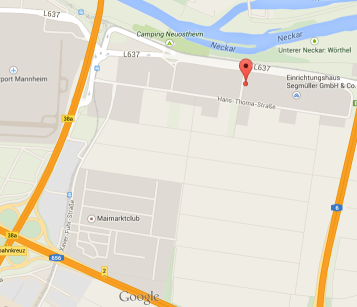
\includegraphics[width=0.3\textwidth]{ref/images/KartenmaterialKlein.png} \\ 
\hline
	\end{tabular}
\end{center}
\caption{Bedeutung von Kartenmaterial} \label{BedeutungVonKartenmaterial}
\end{table}



\subsection{Google Maps}

\subsection{Bing Maps}

\subsection{Open Street Maps}


	\subsubsection{Aufzählen vieler Anwendungsbeispiele mit Erläuterung des Nutzens}
...
	\subsubsection{Umsetzungsmöglichkeiten für die Beispiele nennen}
...
\section{Prototyp}
Prototyp
	\subsection{Auswahl eines Beispiels für einen Prototyp}
...
	\subsection{Nutzen und Ziel der Anwendung}
...
	\subsection{Umsetzung für mobile Endgeräte}
...
	\subsection{Technologie zur Umsetzung}
...
	\subsection{Implementierung}
...
\section{Fazit und Ausblick}
Abschluss
	\subsection{Genereller Ausblick und Fazit für LBS}
...
	\subsection{Speziell auf unsere Anwendung bezogener Ausblick + Fazit}
...
\pagenumbering{roman}

\clearpage
\newpage 

\singlespacing

\opt{bib}{
	\phantomsection
	\headAndTocENDE{References}{Literatur}
	\bibliography{ref/bib}{} 
	\bibliographystyle{phcpcDE}
}
%\opt{appendix}{
%	\appendix
%	\head{\nouppercase{\leftmark}}
%	\opt{en}{\pdfbookmark[0]{Appendix}{appendix}}
%	\opt{de}{\pdfbookmark[0]{Anhang}{appendix}}
%	%\section{Appendix sections}

%}

\pagestyle{empty}
%\section*{\reporttype}

\begin{xlist}{xxxxxxxxxxxxxxxxxxxxxxxx} 
  		\item[\textbf{Titel}]        			\reporttitle
		\item[\textbf{Subtitel}]          		\reportsubtitle
		\item[\textbf{Autor}]          			\student
		\item[\textbf{Hochschule}]          	\dhbw
		\item[\textbf{Datum}]          			\handoverdate
		\item[\textbf{Bearbeitungszeitraum}] 	\timerange
		\item[\textbf{Studiengang}]          	\studiengang
		\item[\textbf{Matrikelnummer, Kurs}]  	\matrikel, \kurs
		\item[\textbf{Ausbildungsfirma}]      	\company, \lokation
		\item[\textbf{Betreuer}]   				\tutor
		\item[\textbf{Gutachter}]            	\prof
\end{xlist}
 	
\section*{Abstract}
\begin{abstract}

Im Rahmen dieser Studienarbeit wird zunächst der Begriff eines Location-based Service definiert und auf spezifische Technologien in diesem Zusammenhang eingegangen. Als Verfahren zur Positionsbestimmung werden Satellitenpositionierung, Positionierung in Mobilfunknetzen und Positionsbestimmung in Gebäuden betrachtet. Anschließend werden Anwendungsbereiche und Nutzer vorgestellt. Den praktischen Teil bildet die prototypische Umsetzung einer Location-based Services - Applikation. Bei der Entwicklung werden unter Anderem die Frameworks Cordova, Ionic und Angular-JS eingesetzt.
Das Fazit dieser Arbeit ist, dass Location-based Services eine große Zukunft haben und schon der einfach gehaltene Prototyp mit den gewählten und leicht zu erlernenden Technologien erfolgreich umgesetzt werden kann. Die Präzision der Positionsbestimmung kann mithilfe der iBeacon-Technik weiter erhöht werden.
\end{abstract}



\end{document}